\documentclass[conference]{IEEEtran}
\IEEEoverridecommandlockouts

\usepackage{cite}
\usepackage{amsmath,amssymb,amsfonts}
\usepackage{algorithmic}
\usepackage{graphicx}
\usepackage{textcomp}
\usepackage{xcolor}
\def\BibTeX{{\rm B\kern-.05em{\sc i\kern-.025em b}\kern-.08em
    T\kern-.1667em\lower.7ex\hbox{E}\kern-.125emX}}
\begin{document}

\title{Loosely Coupled GNSS / 3D RISS Integration}

\author{\IEEEauthorblockN{Mazen Elaraby}
\IEEEauthorblockA{\textit{Department of Electrical and Computer Engineering} \\
\textit{Queen's University}\\
Kingston, Canada 
}}

\maketitle

\begin{abstract}
Inertial Navigation Systems (INS) are fundamental to modern navigation, playing a critical role in various industries, including autonomous vehicles, aerial and ground robotics, and geospatial surveying. While advancements in alternative navigation modalities such as vision, LiDAR, and radar have contributed to the field, each suffers from inherent limitations, including environmental dependencies and cost constraints. INS, on the other hand, provides continuous navigation capability independent of external conditions but is prone to long-term drift due to its reliance on dead reckoning. Global Navigation Satellite Systems (GNSS) offer absolute positioning with high accuracy, yet they are susceptible to jamming, spoofing, and signal degradation in challenging environments.

The fusion of INS and GNSS mitigates these individual shortcomings, creating a robust navigation solution that leverages the short-term accuracy of INS and the long-term stability of GNSS. In this work, we present a loosely coupled integration of a 3D Reduced Inertial Sensor System (RISS) with GNSS, designed to enhance navigation reliability. We describe the implementation details of this integration and analyze its performance under various conditions. Furthermore, we investigate the impact of GNSS outages on the navigation solution, demonstrating the system's ability to maintain accuracy in degraded GNSS environments. The results highlight the effectiveness of 3D RISS/GNSS fusion in achieving a balance between robustness and precision, making it a viable approach for resilient navigation in real-world applications.
\end{abstract}

\begin{IEEEkeywords}
Inertial Navigation System (INS), Global Navigation Satellite System (GNSS), Reduced Inertial Sensor System (RISS), Sensor Fusion, Loosely Coupled Integration, Dead Reckoning, GNSS Outages, Navigation, Autonomous Vehicles, Positioning and Localization.
\end{IEEEkeywords}

\section{Introduction}
Inertial Navigation Systems (INS) have become indispensable in modern navigation, finding applications across a wide range of industries, including aerial and ground robotics, autonomous vehicles, surveying, and defense systems. Their ability to provide continuous navigation solutions without reliance on external signals makes them particularly useful in challenging environments where other navigation systems may struggle. From guiding unmanned aerial vehicles (UAVs) through GPS-denied environments to enabling precise geospatial mapping in surveying applications, INS plays a pivotal role in contemporary positioning and navigation solutions.

As the field of navigation technology progresses, various sensor modalities such as vision, LiDAR, and radar have gained traction in enhancing localization capabilities. Vision-based navigation has demonstrated remarkable success in structure-rich environments but remains susceptible to varying lighting conditions, adverse weather, and featureless terrains. LiDAR-based systems offer high-resolution spatial awareness but are hindered by environmental conditions such as rain, fog, and snow, in addition to their high cost. Similarly, radar-based navigation, though robust against weather disturbances, suffers from limited angular resolution, which constrains its precision in certain applications.

In contrast, inertial sensors have remained a cornerstone of navigation due to their self-contained nature, providing continuous motion tracking independent of external signals. Unlike other modalities, they are immune to environmental changes and operate reliably across diverse conditions. However, their reliance on dead reckoning—a process that accumulates small errors over time—leads to significant drift, ultimately degrading their accuracy over extended durations.

To counteract this drift, Global Navigation Satellite Systems (GNSS) offer an absolute reference solution with meter-level accuracy, which can be further refined to centimeter-level precision using techniques such as Real-Time Kinematic (RTK) and Precise Point Positioning (PPP). Despite their high accuracy, GNSS signals are vulnerable to jamming, spoofing, and multipath errors, and they typically operate at a lower data rate than inertial sensors.

The fusion of INS and GNSS forms an ideal complementary system, as GNSS corrects the drift inherent in INS, while INS provides high-rate updates that bridge the gap between GNSS position fixes. This synergy has established INS/GNSS integration as a reliable and robust navigation solution across multiple domains.

This work aims to develop and implement a loosely coupled integration between a 3D Reduced Inertial Sensor System (RISS) and GNSS. We begin by reviewing the implementation details of this integration approach, followed by an evaluation of its performance. Additionally, we analyze the impact of GNSS outages on the overall navigation solution, highlighting the system's resilience and limitations in real-world conditions.

\section{Implementation Details}
\subsection{System Overview}

The 3D Reduced Inertial Sensor System (RISS) and GNSS integration follows a \textbf{loosely coupled architecture} Figure~\ref{fig:BD}, wherein the two subsystems operate independently and their outputs are fused at the position and velocity levels to enhance overall navigation accuracy. This fusion framework leverages the complementary characteristics of inertial sensors and GNSS, ensuring robust performance across a variety of operating conditions.

\begin{figure}[htbp]
\centerline{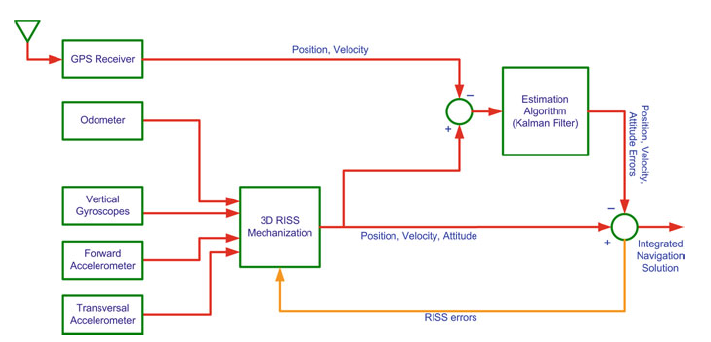
\includegraphics[width=0.48\textwidth]{BD.png}}
\caption{A block diagram of a loosely coupled 3D RISS/GPS integration}
\label{fig:BD}
\end{figure}

\subsubsection{Sensor Inputs and Mechanization}
The 3D RISS subsystem forms the core of the system, utilizing a set of self-contained inertial sensors to estimate position, velocity, and attitude. This subsystem consists of:

\begin{itemize}
    \item A \textbf{vertical gyroscope}, responsible for measuring angular rate about the vertical axis, thereby aiding in heading estimation.
    \item A \textbf{forward accelerometer}, which captures linear acceleration in the vehicle’s primary motion direction.
    \item A \textbf{transversal accelerometer}, used to measure lateral motion, further refining position and velocity estimates.
    \item An \textbf{odometer}, which provides vehicle's speed in forward direction.
\end{itemize}

The RISS mechanization process continuously integrates acceleration and angular rate data to compute real-time position, velocity, and attitude. However, as the system relies on dead reckoning, small sensor errors accumulate over time, leading to drift, which degrades accuracy in long-term navigation.

\subsubsection{GNSS Integration and Error Estimation}
To mitigate the inherent drift of RISS, a GNSS receiver provides \textbf{absolute position and velocity measurements}. GNSS-based navigation, while highly accurate in open-sky conditions, suffers from signal loss, multipath errors, jamming, and spoofing, making it unreliable in urban environments, tunnels, or GNSS-denied areas. Additionally, GNSS typically operates at a lower data rate compared to inertial sensors, resulting in gaps between position updates.

To optimally integrate these two subsystems, a Kalman filter-based estimation algorithm is employed. The Kalman filter functions as a recursive estimator, continuously comparing the GNSS-derived position and velocity with those obtained from the RISS mechanization process. The filter then computes position, velocity, and attitude errors, which are fed back into the system to refine the final navigation solution.

The final integrated navigation solution is derived by compensating for the drift in RISS using GNSS corrections while allowing RISS to provide high-frequency updates between successive GNSS fixes. 

By leveraging this loosely coupled integration approach, the system provides a reliable and resilient navigation framework that combines the strengths of both INS and GNSS.

\subsection{Error-State Vector}

The error-state vector that will be used by the Kalman filter is defined as:

\begin{equation}
\delta x_k = \begin{bmatrix} 
\delta \varphi_k, \delta \lambda_k, \delta h_k, \delta v_k^E, \delta v_k^N, \delta v_k^U, \delta A_k, SF_k^{od}, \delta \omega_k^z
\end{bmatrix}^T
\end{equation}

where:

\begin{itemize}
    \item $\delta \varphi_k$ \quad is the error in latitude.
    \item $\delta \lambda_k$ \quad is the error in longitude.
    \item $\delta h_k$ \quad is the error in altitude.
    \item $\delta v_k^E$ \quad is the error in the velocity component along the east direction.
    \item $\delta v_k^N$ \quad is the error in the velocity component along the north direction.
    \item $\delta v_k^U$ \quad is the error in the velocity component along the up direction.
    \item $\delta A_k$ \quad is the error in the azimuth angle.
    \item $SF_k^{od}$ \quad is the scale factor error of the odometer-derived speed.
    \item $\delta \omega_k^z$ \quad is the stochastic gyroscope drift.
\end{itemize}

\subsection{Stochastic Modeling of Inertial Sensor Errors}

In most Kalman filter (KF) implementations, the sensor noise portion of the state transition matrix $F$ is based on a first-order Gauss-Markov (GM) model \cite{iqbal2009}. 

\subsubsection{The Gauss-Markov Process}

A stationary Gaussian process $x(t)$ that has an exponential autocorrelation is called a Gauss-Markov (GM) process. The statistics of a stationary GM process are completely described by its autocorrelation function as follows:

\begin{equation}
    R_{xx}(\tau) = \sigma^2 e^{-\beta |\tau|}
\end{equation}

where $\sigma^2$ is the variance of the sensor noise, and $\beta$ is the reciprocal of the correlation time, which corresponds to a decaying exponential autocorrelation sequence.

A first-order Gauss-Markov process $x(t)$ is described as follows:

\begin{equation}
    \dot{x}(t) = -\beta x(t) + \sqrt{2\sigma^2 \beta} w(t),
    \label{eq:gm_continuous}
\end{equation}

where $w(t)$ is modeled as unity variance white Gaussian noise. By computing the autocorrelation function, the variance $(\sigma^2)$ can be determined from the maximum value, and the correlation time $(\tau)$ can be calculated from the time corresponding to $(1/e)\sigma^2$. These parameters are determined from actual experimental data from a stationary run.

In discrete-time domain, Equation~\eqref{eq:gm_continuous} is written as:

\begin{equation}
    x_k = (I - \beta \Delta t) x_{k-1} + \sqrt{2\beta \sigma^2} w_k \Delta t,
\end{equation}

where $\Delta t$ is the sampling interval.

\subsection{System Model of the Kalman Filter}

A non-linear motion model forms the basis of mechanization, and the linearized error-state model derived from this serves as the system model for a Kalman filter.

As mentioned, the motion model is non-linear and must be linearized to obtain the error model that will serve as the system model for the Kalman filter. These equations are linearized by applying a Taylor series expansion and ignoring the higher-order terms. The corresponding linearized error-state system model is therefore given by \cite{noureldin2013}:

\begin{equation}
    \boldsymbol{\delta x}_k = 
    \begin{bmatrix} 
        \boldsymbol{\delta r}_k \\ 
        \boldsymbol{\delta v}_k \\ 
        \boldsymbol{\delta e}_k 
    \end{bmatrix} =
    \begin{bmatrix} 
        \mathbf{I}_{3\times3} & \mathbf{F}_1 & \mathbf{0}_{3\times3} \\ 
        \mathbf{0}_{3\times3} & \mathbf{I}_{3\times3} & \mathbf{F}_2 \\ 
        \mathbf{0}_{3\times3} & \mathbf{0}_{3\times3} & \mathbf{F}_3 
    \end{bmatrix}
    \begin{bmatrix} 
        \boldsymbol{\delta r}_{k-1} \\ 
        \boldsymbol{\delta v}_{k-1} \\ 
        \boldsymbol{\delta e}_{k-1} 
    \end{bmatrix}
    + 
    \begin{bmatrix} 
        \mathbf{0}_{3\times1} \\ 
        \mathbf{0}_{3\times1} \\ 
        \boldsymbol{\sigma} 
    \end{bmatrix}
    \label{eq:error_state_system}
\end{equation}

where:

\begin{equation}
    \boldsymbol{\delta r}_k =
    \begin{bmatrix} 
        \delta \varphi_k \\ 
        \delta \lambda_k \\ 
        \delta h_k 
    \end{bmatrix}
\end{equation}

\begin{equation}
    \boldsymbol{\delta v}_k =
    \begin{bmatrix} 
        \delta v_k^E \\ 
        \delta v_k^N \\ 
        \delta v_k^U 
    \end{bmatrix}
\end{equation}

\begin{equation}
    \boldsymbol{\delta e}_k =
    \begin{bmatrix} 
        \delta A_k \\ 
        SF_k^{od} \\ 
        \delta \omega_k^z 
    \end{bmatrix}
\end{equation}

\begin{equation}
    \boldsymbol{\delta \sigma}_k =
    \begin{bmatrix} 
        0 \\ 
        \sqrt{2 \gamma_{od} \sigma_{od}^2 \Delta t} \\ 
        \sqrt{2 \beta_z \sigma_z^2 \Delta t} 
    \end{bmatrix}
\end{equation}

The transition matrices $\mathbf{F}_1$, $\mathbf{F}_2$, and $\mathbf{F}_3$ are defined as follows:

\begin{equation}
    \mathbf{F}_1 =
    \begin{bmatrix} 
        0 & 0 & 0 \\ 
        \frac{1}{(R_N+h_{k-1}) \cos{\varphi_{k-1}}} \Delta t & 0 & 0 \\ 
        \frac{1}{R_M+h_{k-1}} \Delta t & 0 & 0 
    \end{bmatrix}
\end{equation}

\begin{equation}
    \mathbf{F}_2 =
    \begin{bmatrix} 
        v_{k-1}^{od} \cos A_{k-1} \cos p_{k-1} & v_{k-1}^{od} \sin A_{k-1} \cos p_{k-1} & 0 \\ 
        -v_{k-1}^{od} \sin A_{k-1} \cos p_{k-1} & v_{k-1}^{od} \cos A_{k-1} \cos p_{k-1} & 0 \\ 
        0 & v_{k-1}^{od} \sin p_{k-1} & 0 
    \end{bmatrix}
\end{equation}

\begin{equation}
    \mathbf{F}_3 =
    \begin{bmatrix} 
        1 & 0 & -\Delta t \\ 
        0 & 1 - \gamma_{od} \Delta t & 0 \\ 
        0 & 0 & 1 - \beta_z \Delta t 
    \end{bmatrix}
\end{equation}

The stochastic errors associated with the gyroscope and the odometer-derived speed are modeled by a Gauss-Markov process, where $\gamma_{od}$ is the reciprocal of the autocorrelation time for the scale factor of the odometer-derived speed, $\sigma_{od}^2$ is the variance of the noise associated with it, $\beta_z$ is the reciprocal of the autocorrelation time for the gyroscope's stochastic drift, and $\sigma_z^2$ is the variance of the noise associated with it.

\subsection{Measurement Model of the Kalman Filter}

Since we are considering loosely coupled integration, GPS position and velocity updates are used during the update stage of the Kalman filter (KF). The measurement model used by the filter is given by:

\begin{equation}
    \boldsymbol{\delta z}_k =
    \begin{bmatrix}
        \varphi_k^{RISS} - \varphi_k^{GPS} \\
        \lambda_k^{RISS} - \lambda_k^{GPS} \\
        h_k^{RISS} - h_k^{GPS} \\
        v_{k}^{E,RISS} - v_{k}^{E,GPS} \\
        v_{k}^{N,RISS} - v_{k}^{N,GPS} \\
        v_{k}^{U,RISS} - v_{k}^{U,GPS}
    \end{bmatrix}
    = \mathbf{H} \boldsymbol{\delta x}_k + \boldsymbol{\delta \eta}_k
    \label{eq:measurement_model}
\end{equation}

where $\boldsymbol{\delta z}_k$ represents the difference between the 3D positions and velocities estimated by RISS mechanization and those provided by GPS, and $\boldsymbol{\delta \eta}_k$ is the measurement noise.

Expanding the measurement equation, we obtain:

\begin{equation}
    \boldsymbol{\delta z}_k =
    \begin{bmatrix}
        1 & 0 & 0 & 0 & 0 & 0 & 0 & 0 & 0 \\
        0 & 1 & 0 & 0 & 0 & 0 & 0 & 0 & 0 \\
        0 & 0 & 1 & 0 & 0 & 0 & 0 & 0 & 0 \\
        0 & 0 & 0 & 1 & 0 & 0 & 0 & 0 & 0 \\
        0 & 0 & 0 & 0 & 1 & 0 & 0 & 0 & 0 \\
        0 & 0 & 0 & 0 & 0 & 1 & 0 & 0 & 0
    \end{bmatrix}
    \begin{bmatrix}
        \delta \varphi_k \\
        \delta \lambda_k \\
        \delta h_k \\
        \delta v_k^E \\
        \delta v_k^N \\
        \delta v_k^U \\
        \delta A_k \\
        SF_k^{od} \\
        \delta \omega_k^z
    \end{bmatrix}
    + 
    \begin{bmatrix}
        \delta \eta_k^\varphi \\
        \delta \eta_k^\lambda \\
        \delta \eta_k^h \\
        \delta \eta_k^{vE} \\
        \delta \eta_k^{vN} \\
        \delta \eta_k^{vU}
    \end{bmatrix}
    \label{eq:measurement_expansion}
\end{equation}

This formulation expresses how GPS measurements are incorporated into the Kalman filter update stage. The measurement matrix $\mathbf{H}$ acts as a selector, mapping the error state vector $\boldsymbol{\delta x}_k$ to the observed measurement residuals. The measurement noise vector $\boldsymbol{\delta \eta}_k$ accounts for uncertainties in the GPS updates.

\subsection{Kalman Filter Equations}

The Kalman filter is a recursive estimation algorithm that operates in two main steps: 
\begin{itemize}
    \item \textbf{Prediction step:} The state and covariance are propagated forward based on the system dynamics.
    \item \textbf{Correction step:} The predicted state is corrected using new measurement updates to reduce uncertainty.
\end{itemize}

For the \textbf{error-state Kalman filter}, the estimation process is governed by the following equations:

\subsubsection{Prediction Step}
\textbf{State Vector Prediction:}  
\begin{equation}
    \boldsymbol{\delta \hat{x}}_k^{-} = \mathbf{\Phi}_{k-1} \boldsymbol{\delta \hat{x}}_{k-1}^{+}
    \label{eq:kf_state_prediction}
\end{equation}

\textbf{Covariance Prediction:}  
\begin{equation}
    \mathbf{P}_k^{-} = \mathbf{\Phi}_{k-1} \mathbf{P}_{k-1}^{+} \mathbf{\Phi}_{k-1}^{T} + \mathbf{G}_{k-1} \mathbf{Q}_{k-1} \mathbf{G}_{k-1}^{T}
    \label{eq:kf_cov_prediction}
\end{equation}

\subsubsection{Correction Step}
\textbf{Kalman Gain Calculation:}  
\begin{equation}
    \mathbf{K}_{k} = \mathbf{P}_k^{-} \mathbf{H}_k^{T} \left(\mathbf{H}_k \mathbf{P}_k^{-} \mathbf{H}_k^{T} + \mathbf{R}_k \right)^{-1}
    \label{eq:kf_gain}
\end{equation}

\textbf{State Estimate Update:}  
\begin{equation}
    \boldsymbol{\delta \hat{x}}_k^{+} = \boldsymbol{\delta \hat{x}}_k^{-} + \mathbf{K}_k \left(\boldsymbol{\delta z}_k - \mathbf{H}_k \boldsymbol{\delta \hat{x}}_k^{-} \right)
    \label{eq:kf_state_update}
\end{equation}

\textbf{Covariance Update:}  
\begin{equation}
    \mathbf{P}_k^{+} = \mathbf{P}_k^{-} - \mathbf{K}_k \mathbf{H}_k \mathbf{P}_k^{-}
    \label{eq:kf_cov_update}
\end{equation}

where:
\begin{itemize}
\item $\boldsymbol{\delta \hat{x}}_k^{-}$ is the predicted error-state vector.
\item $\boldsymbol{\delta \hat{x}}_k^{+}$ is the updated error-state vector after measurement correction.
\item $\mathbf{\Phi}_{k-1}$ is the state transition matrix.
\item $\mathbf{P}_k^{-}$ and $\mathbf{P}_k^{+}$ are the error covariance matrices before and after measurement updates.
\item $\mathbf{G}_{k-1}$ is the process noise coupling matrix.
\begin{equation}
    \mathbf{G} =
    \begin{pmatrix}
        1 & 1 & 1 & 1 & 1 & 1 & \sqrt{2\gamma_{od} \sigma_{od}^2} & \sqrt{2\beta_z \sigma_z^2}
    \end{pmatrix}^{T}.
\end{equation}

\item $\mathbf{Q}_{k-1}$ is the process noise covariance matrix.
\item $\mathbf{H}_k$ is the measurement matrix, mapping the error-state to the measurement domain.
\item $\mathbf{R}_k$ is the measurement noise covariance matrix. The diagonal elements correspond to variances of the GPS
measurements
\begin{equation}
    \mathbf{R} =
    \begin{pmatrix}
        \sigma^2_{\varphi} & 0 & 0 & 0 & 0 & 0 \\
        0 & \sigma^2_{\lambda} & 0 & 0 & 0 & 0 \\
        0 & 0 & \sigma^2_{h} & 0 & 0 & 0 \\
        0 & 0 & 0 & \sigma^2_{V_e} & 0 & 0 \\
        0 & 0 & 0 & 0 & \sigma^2_{V_n} & 0 \\
        0 & 0 & 0 & 0 & 0 & \sigma^2_{V_u}
    \end{pmatrix}.
\end{equation}

\item $\boldsymbol{\delta z}_k$ is the measurement error vector, representing the difference between the observed and estimated measurements.
\item $\mathbf{K}_k$ is the Kalman gain, which determines the weighting of the measurement update.
\end{itemize}

The prediction step propagates the estimated state and its uncertainty forward in time, while the correction step refines the estimate by incorporating new measurement information. This recursive process ensures an optimal estimate of the navigation error states by continuously balancing process dynamics and measurement updates.


\section{Results}

The system was tested using data collected from a single trajectory, covering approximately 12.6 km over a duration of 42 minutes. A lowcost,
automotive-grade MEMS-based IMU (VTI IMU) IMU was used. The speed readings have been obtained through the On-Board Diagnostics version II (OBD II) interface using a device called CarChip.

\begin{figure}[htbp]
\centerline{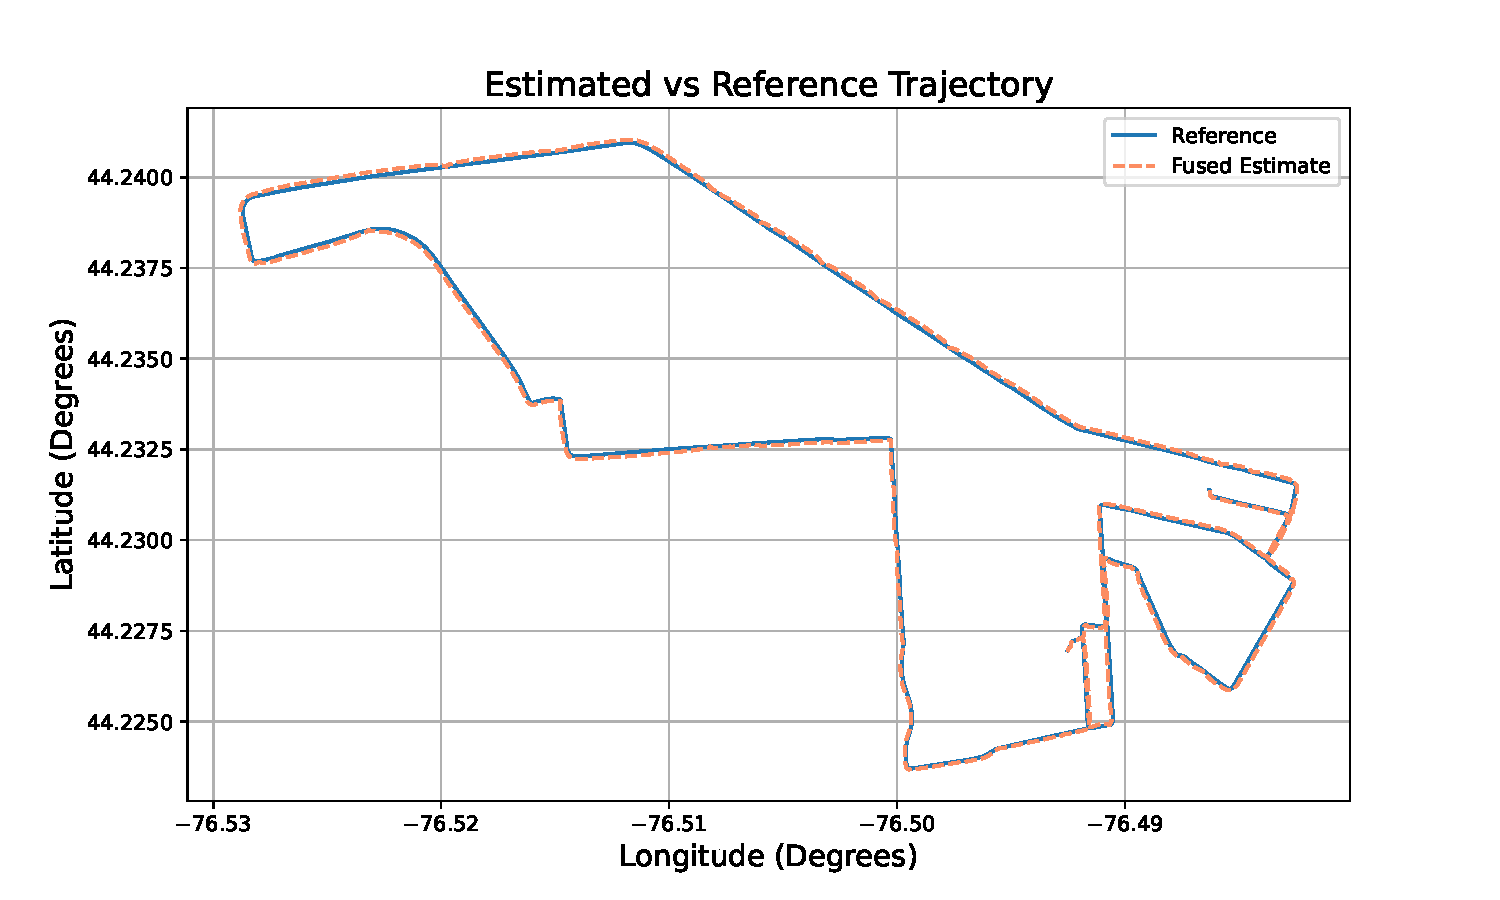
\includegraphics[width=0.48\textwidth]{plots/traj.pdf}}
\caption{Estimated Trajectory}
\label{fig:traj}
\end{figure}

\begin{table*}[h!]
\centering
\begin{tabular}{|c|c|c|c|c|c|c|c|c|c|c|c|c|c|c|c|}
\hline
\textbf{Method} & \multicolumn{3}{c|}{\textbf{North}} & \multicolumn{3}{c|}{\textbf{East}} & \multicolumn{3}{c|}{\textbf{Altitude}} & \multicolumn{3}{c|}{\textbf{2D}} & \multicolumn{3}{c|}{\textbf{3D}} \\
\cline{2-16}
 & \textbf{Std} & \textbf{RMS} & \textbf{Max} & \textbf{Std} & \textbf{RMS} & \textbf{Max} & \textbf{Std} & \textbf{RMS} & \textbf{Max} & \textbf{Std} & \textbf{RMS} & \textbf{Max} & \textbf{Std} & \textbf{RMS} & \textbf{Max} \\
\hline
KF & 5.98 & 5.98 & 16.423 & 5.095 & 5.12 & 15.037 & 0.973 & 1.025 & 7.87 & 5.153 & 7.872 & 19.269 & 5.076 & 7.939 & 19.271 \\
\hline
\end{tabular}
\caption{Error statistics: Std, RMS, and Max for North, East, Altitude, 2D, and 3D Positional Errors.}
\label{tab:error_stats}
\end{table*}

\begin{table*}[h!]
\centering
\begin{tabular}{|c|c|c|c|c|c|c|c|c|c|}
\hline
\textbf{Method} & \multicolumn{3}{c|}{\textbf{East Velocity}} & \multicolumn{3}{c|}{\textbf{North Velocity}} & \multicolumn{3}{c|}{\textbf{Up Velocity}} \\
\cline{2-10}
 & \textbf{Std} & \textbf{RMS} & \textbf{Max} & \textbf{Std} & \textbf{RMS} & \textbf{Max} & \textbf{Std} & \textbf{RMS} & \textbf{Max} \\
\hline
KF & 0.396 & 0.397 & 2.39 & 0.403 & 0.403 & 8.562 & 0.272 & 0.273 & 3.305 \\
\hline
\end{tabular}
\caption{Error statistics: Std, RMS, and Max for East, North and Up Velocity Components Errors.}
\label{tab:velocity_error}
\end{table*}

The following results present the error statistics and performance evaluation of the system in both positioning and velocity estimation, as well as the impact of GPS outages on the navigation solution.

\subsection{Error Statistics in Position and Velocity}

Tables~\ref{tab:error_stats} and \ref{tab:velocity_error} summarize the error statistics (Standard Deviation, RMS, and Maximum) for position and velocity components, respectively. These statistics provide insight into the accuracy of the system under normal operating conditions.

\begin{figure*}[htbp]
\centerline{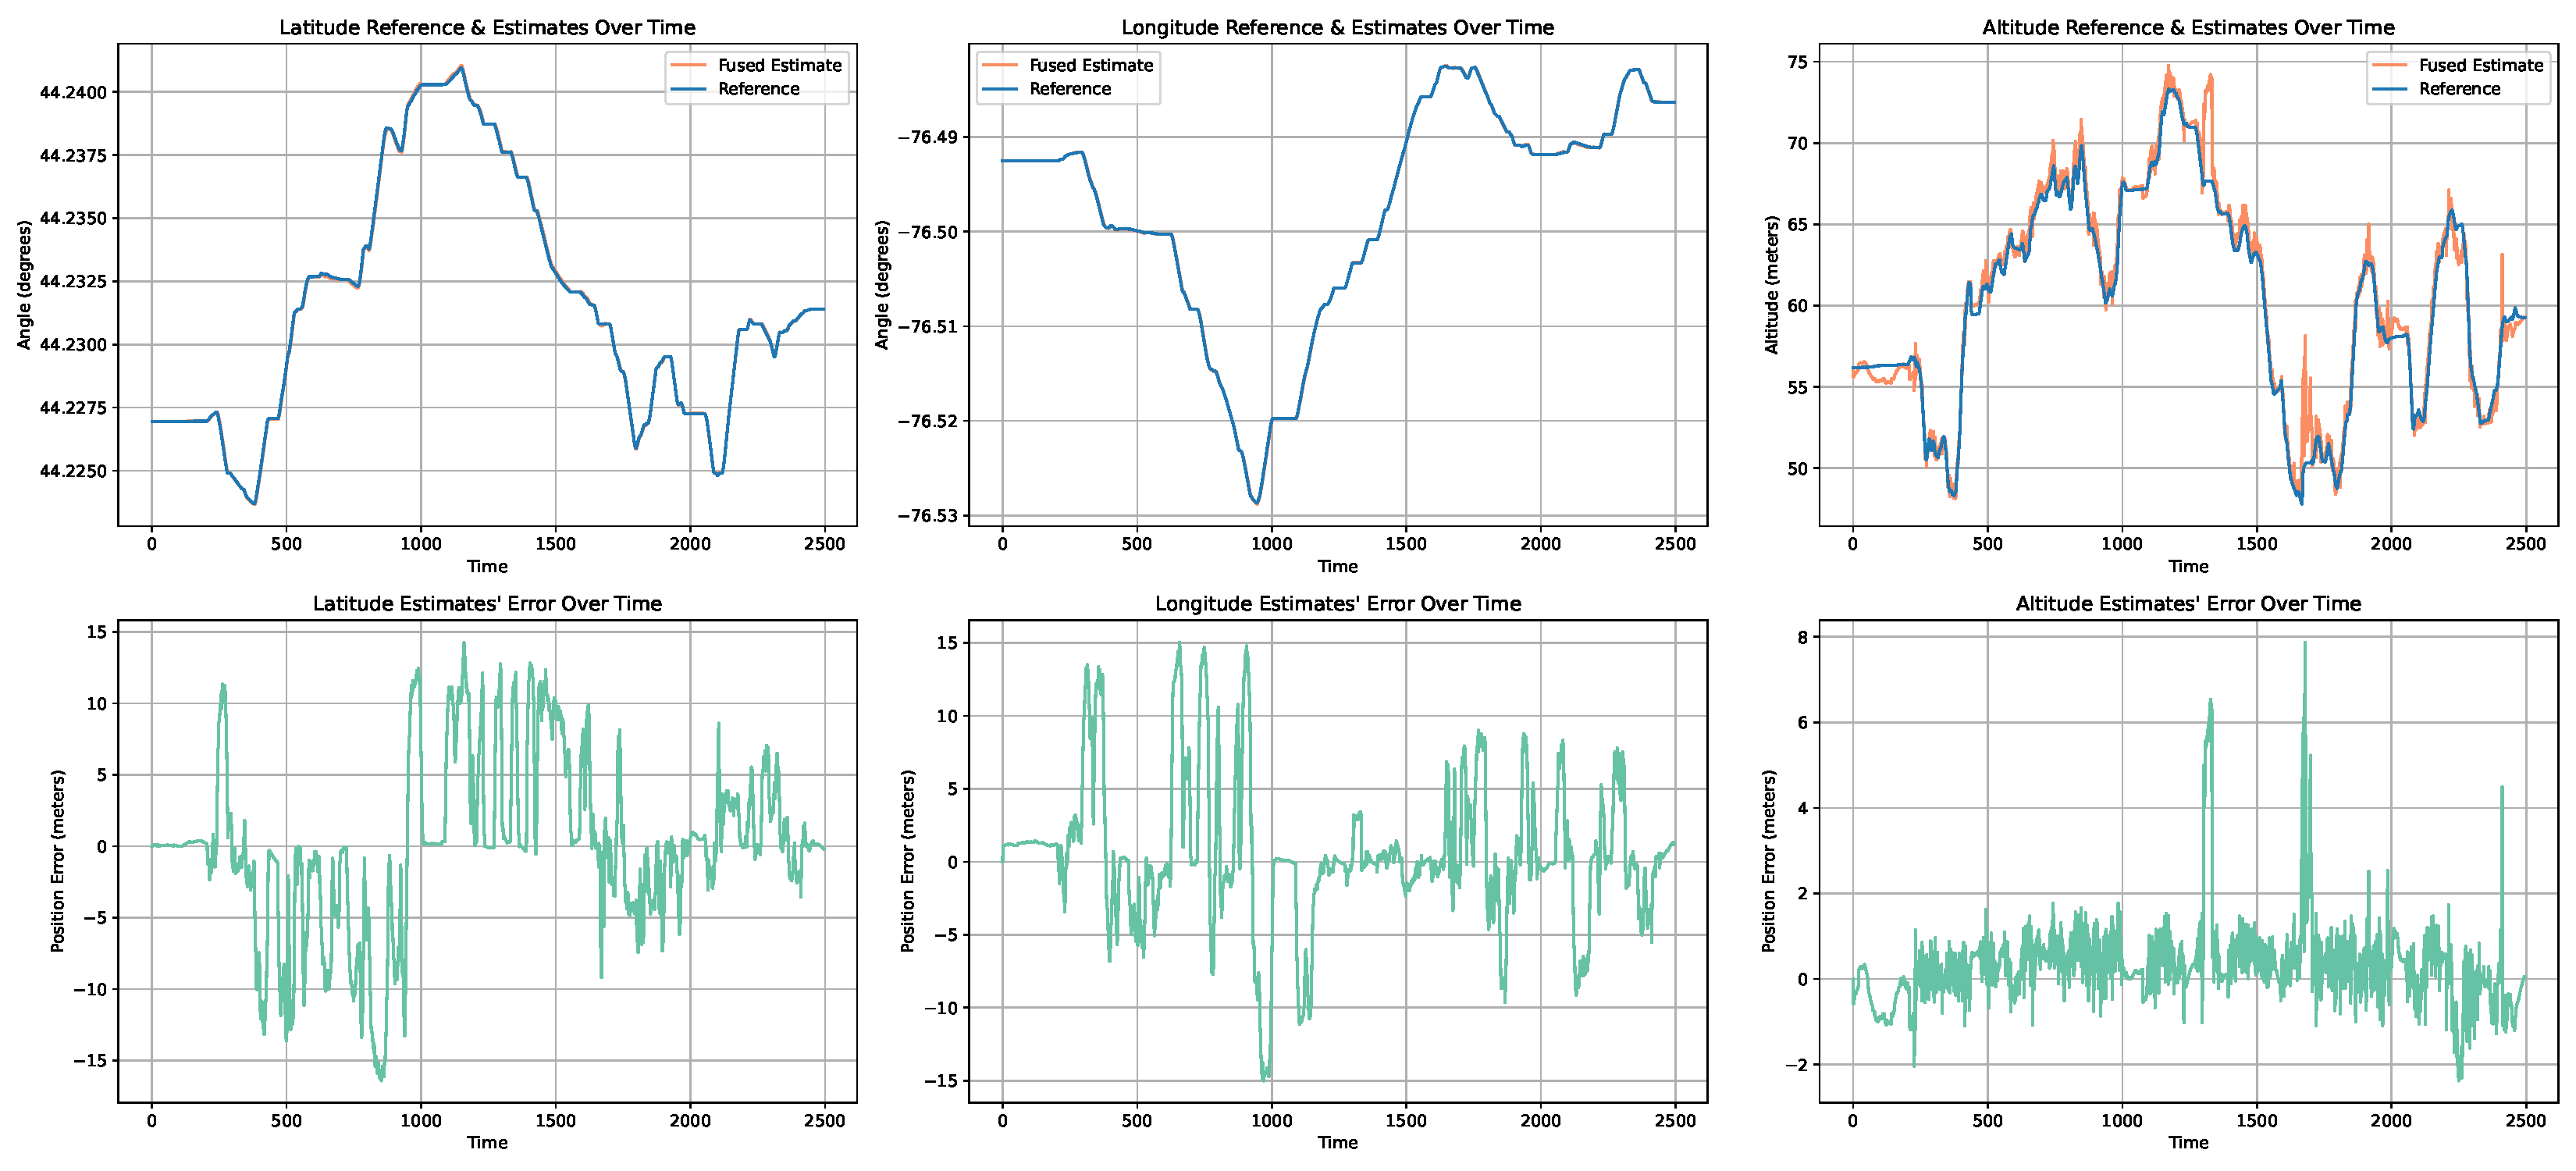
\includegraphics[width=1\textwidth]{plots/pos_err.pdf}}
\caption{Positional Components \& their Associated Errors}
\label{fig:pos_err}
\end{figure*}

\subsection{Positioning Errors}

Figure~\ref{fig:pos_err} illustrates the errors in the three positional components, namely latitude, longitude, and altitude, over time.

\begin{figure*}[htbp]
\centerline{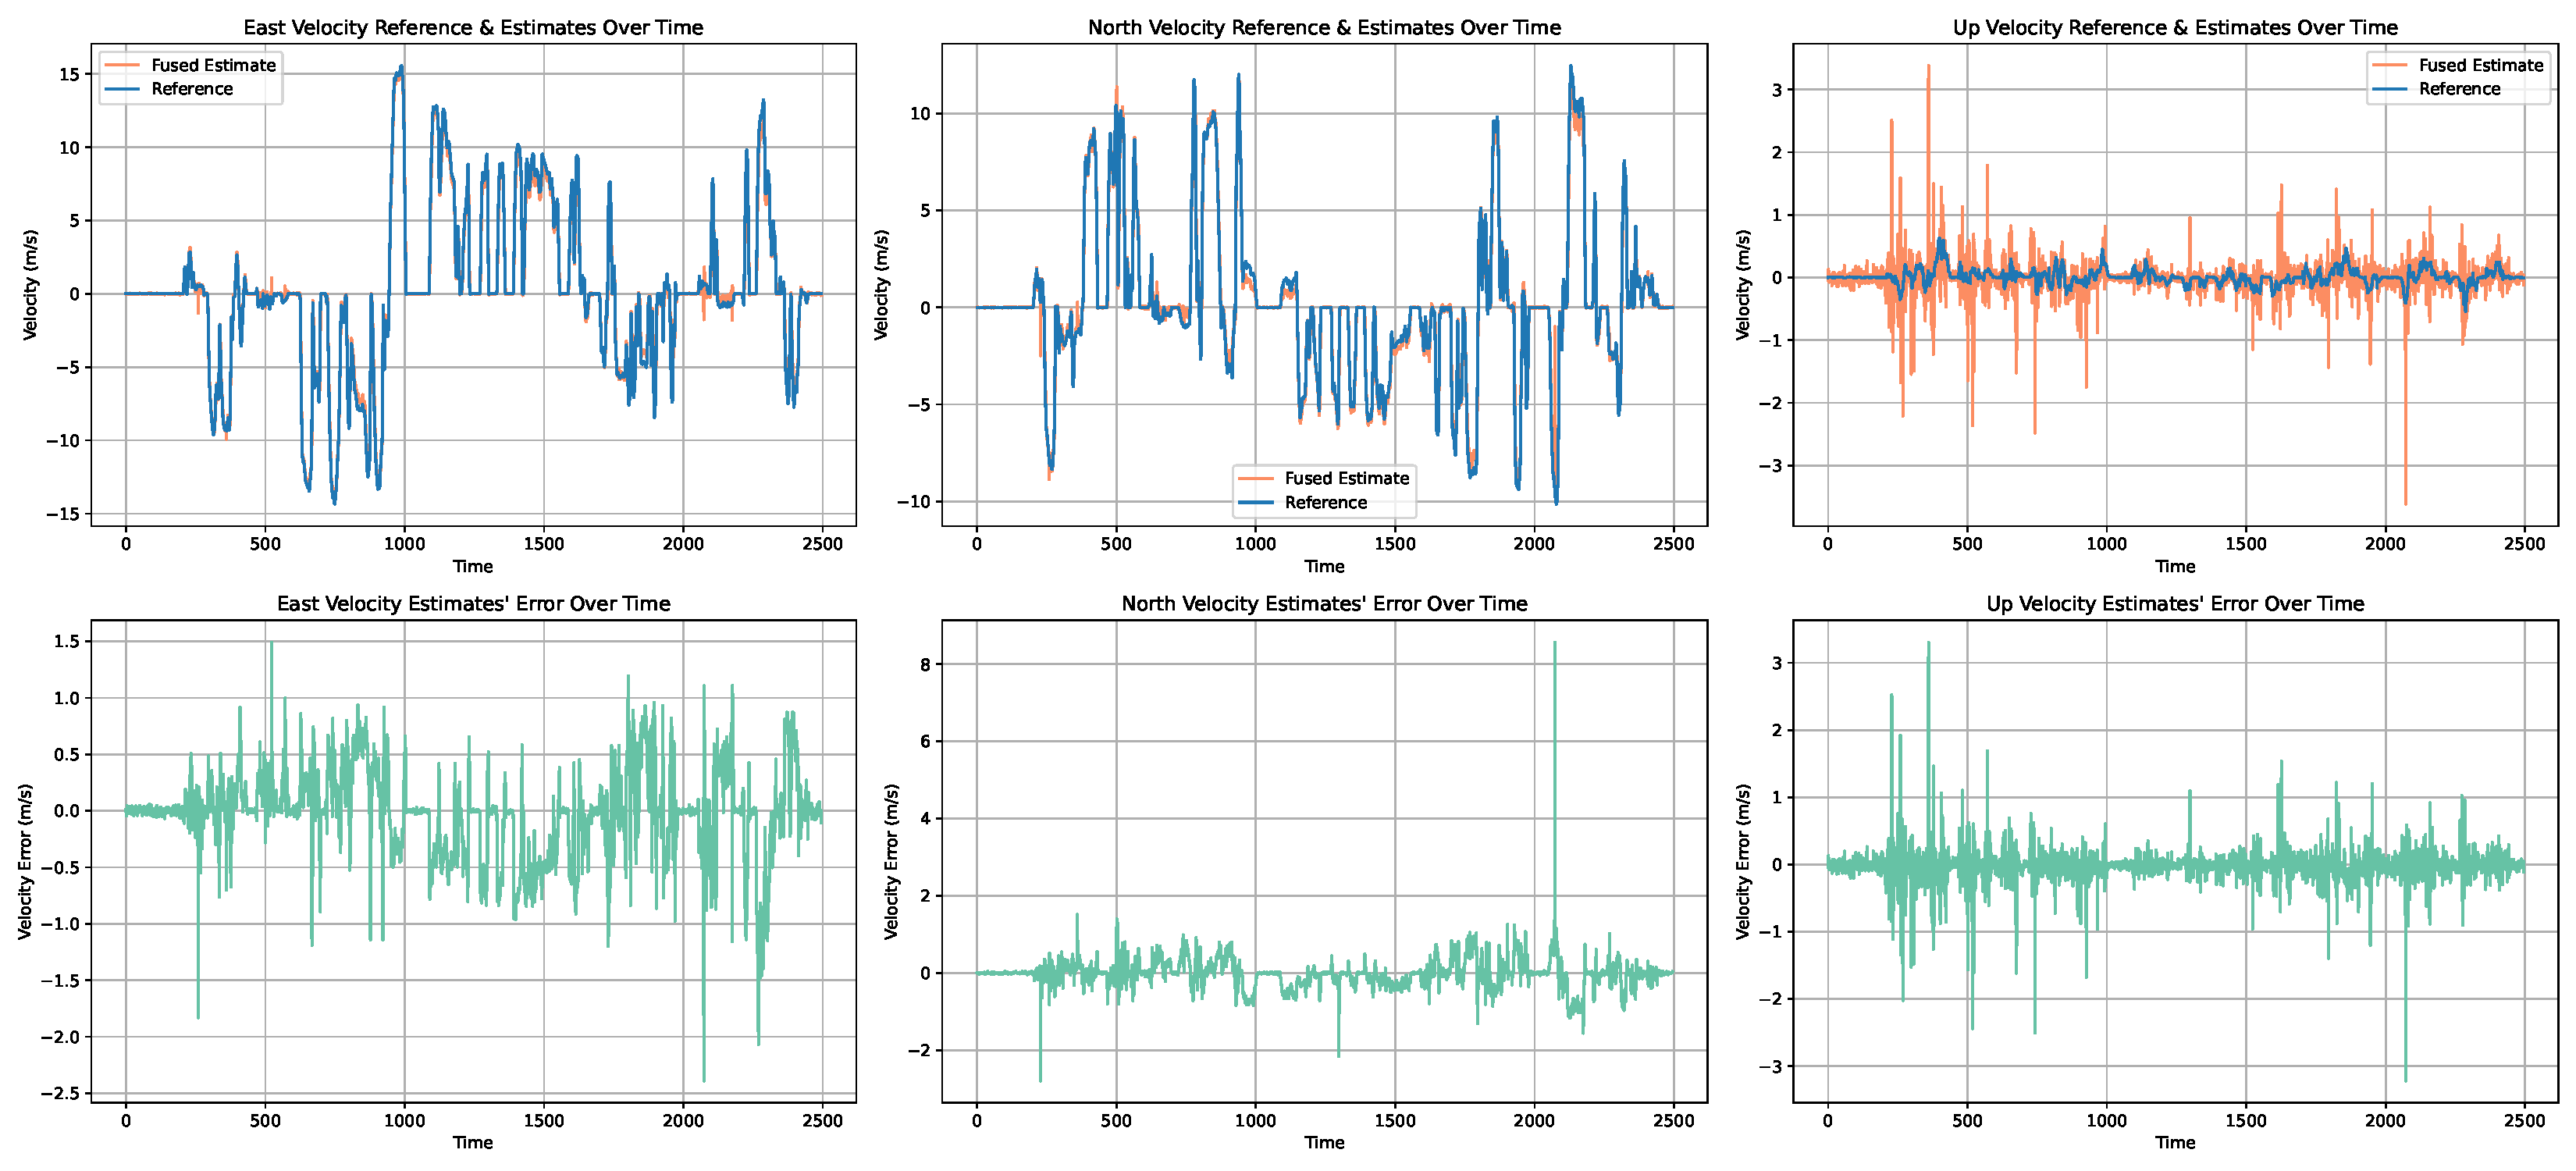
\includegraphics[width=1\textwidth]{plots/vel_err.pdf}}
\caption{Velocity Components \& their Associated Errors}
\label{fig:vel_err}
\end{figure*}

\subsection{Velocity Errors}

The errors in the three velocity components (East velocity, North velocity, and Up velocity) are depicted in Figure~\ref{fig:vel_err}.

\begin{figure}[htbp]
\centerline{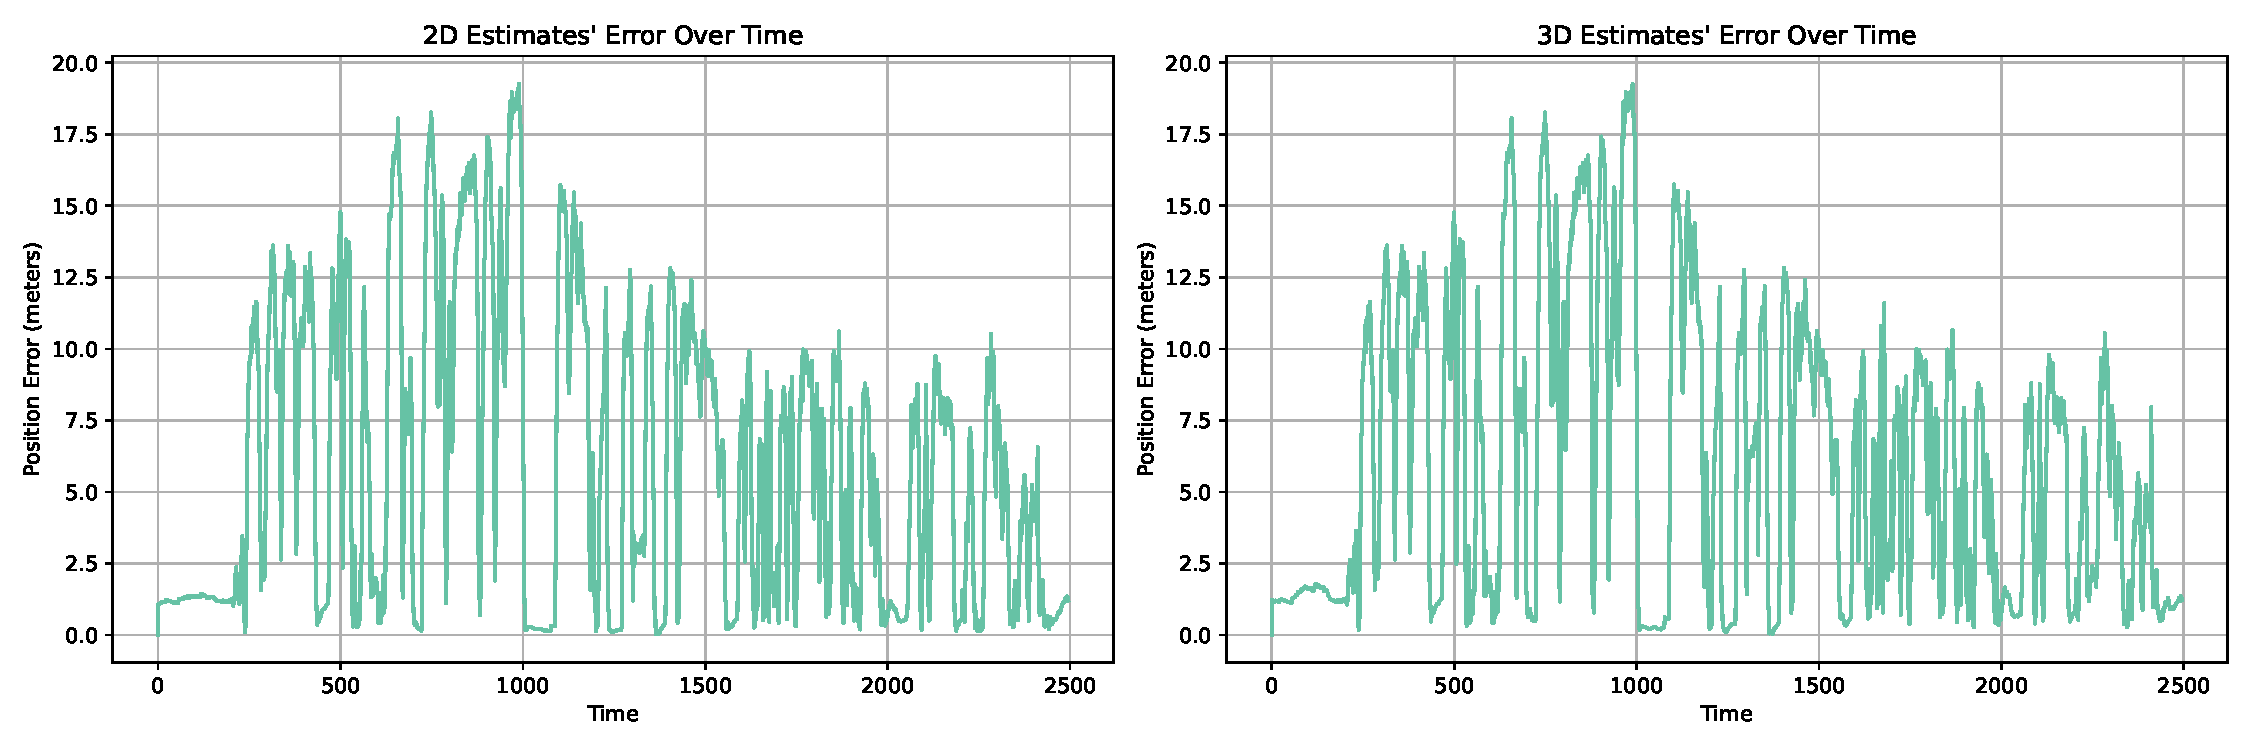
\includegraphics[width=0.48\textwidth]{plots/2D3Derr.pdf}}
\caption{Errors in 2D \& 3D Positioning}
\label{fig:2D3D_err}
\end{figure}

\subsection{2D and 3D Positioning Errors}

Figure~\ref{fig:2D3D_err} presents the errors in 2D and 3D positioning. The 2D positioning error represents the horizontal positioning accuracy, while the 3D positioning error includes vertical components.

\subsection{Effect of GPS Outages on Navigation Accuracy}

To study the impact of GPS outages on system performance, four instances of GPS signal loss were applied:

\begin{itemize}
    \item \textbf{First outage:} 3-minute GPS loss (from 100 to 280 seconds).
    \item \textbf{Second outage:} 2.5-minute GPS loss (from 1000 to 1150 seconds).
    \item \textbf{Third outage:} 1.5-minute GPS loss (from 1500 to 1590 seconds).
    \item \textbf{Fourth outage:} 2-minute GPS loss (from 2000 to 2120 seconds).
\end{itemize}

\begin{figure*}[htbp]
\centerline{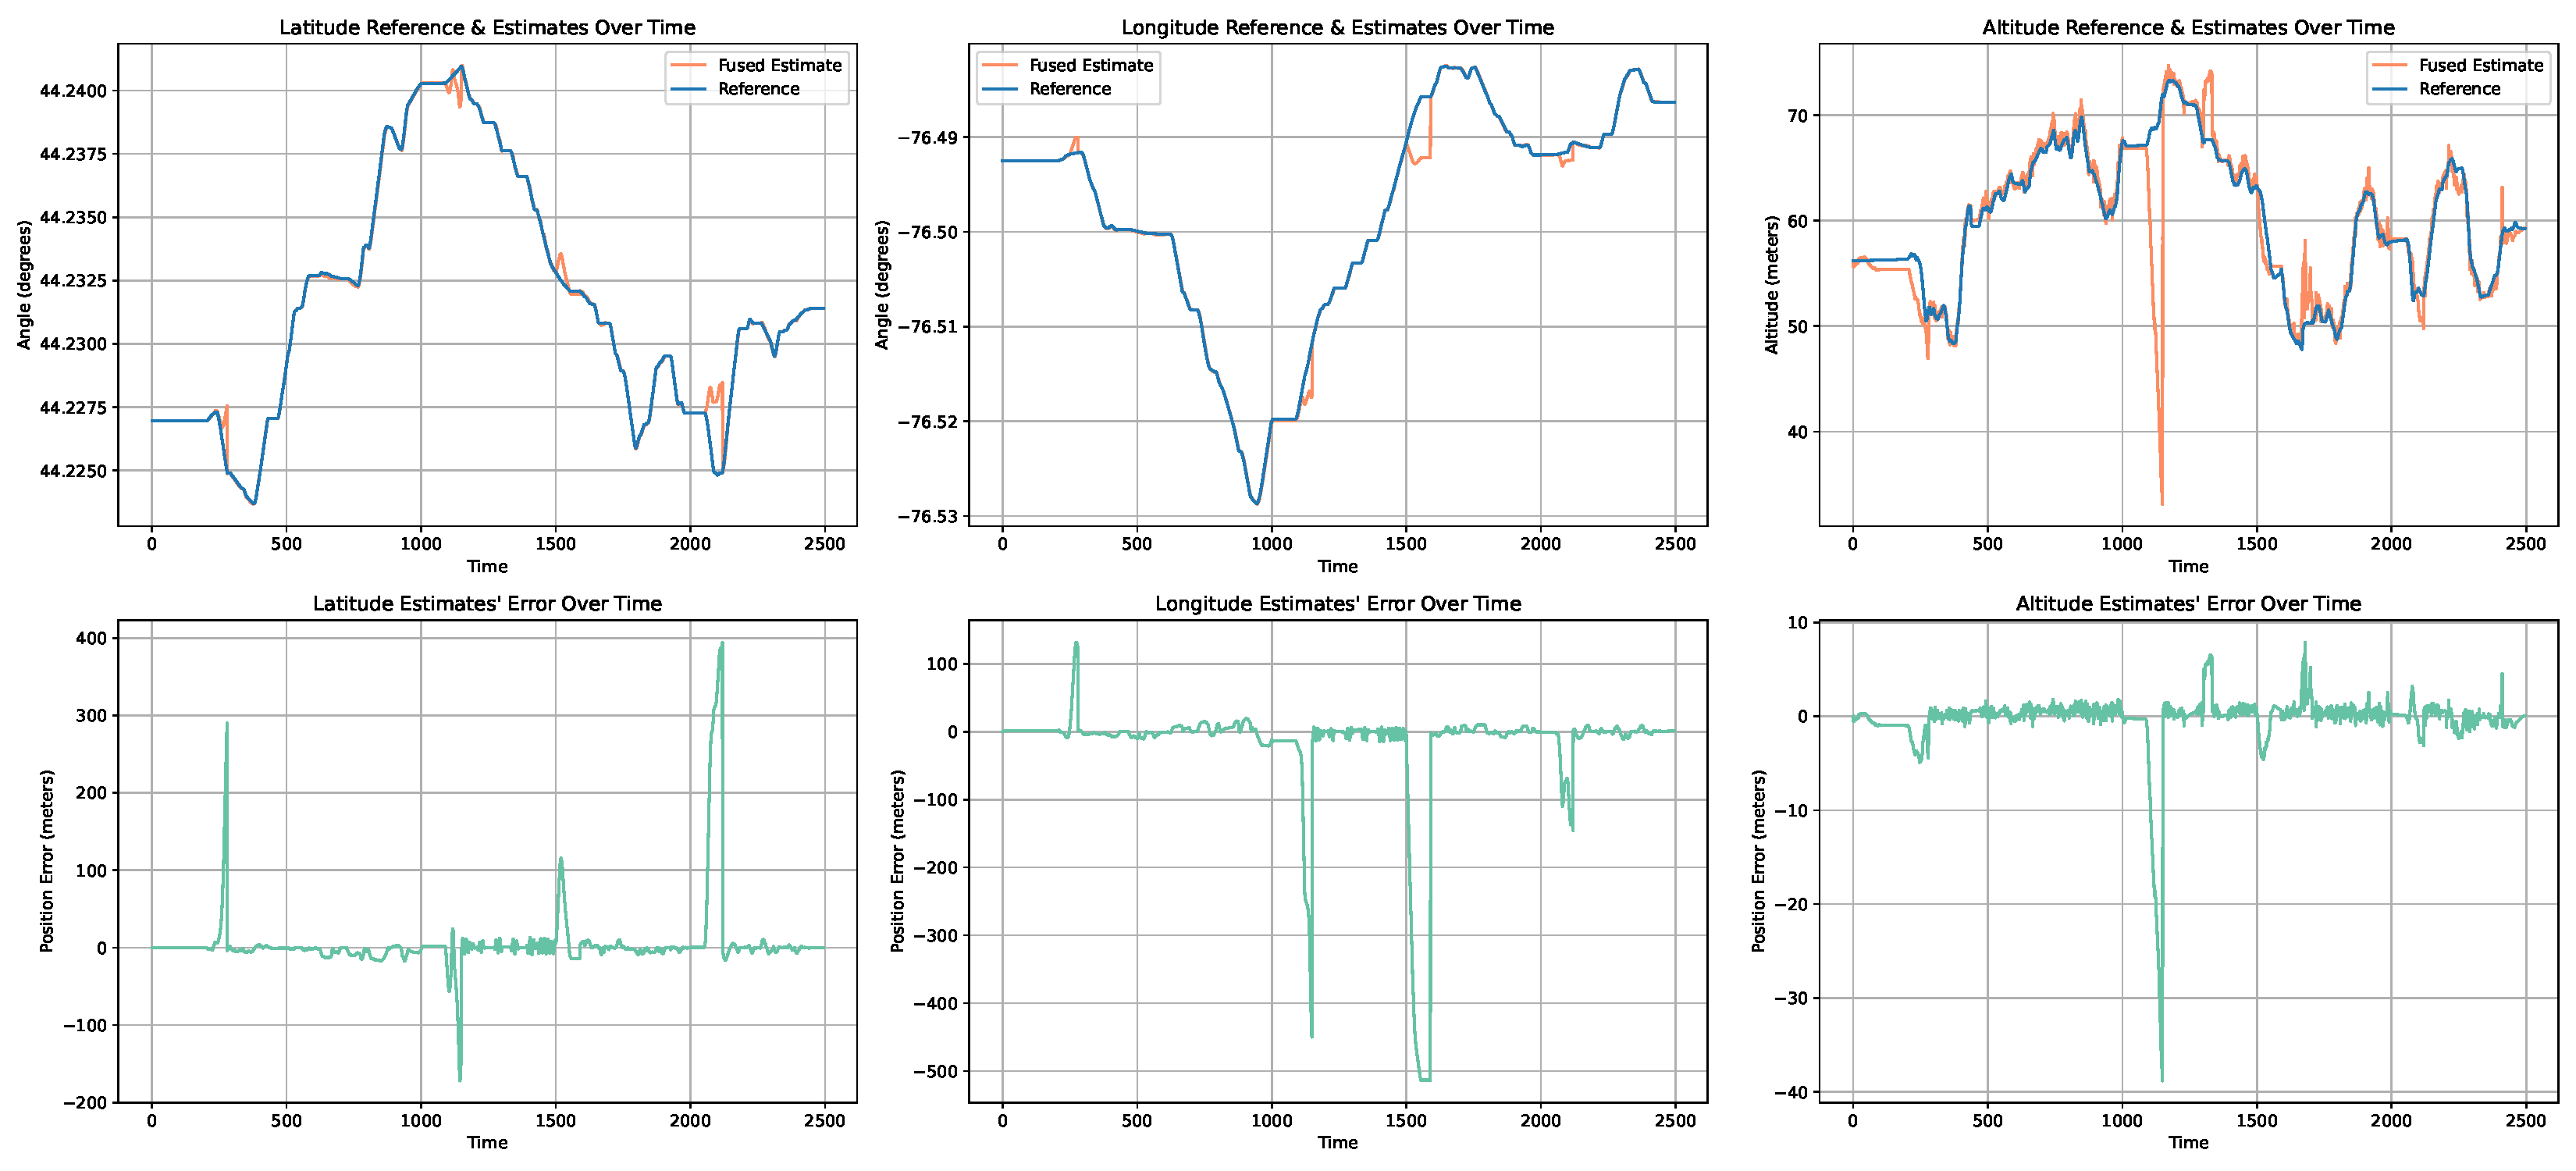
\includegraphics[width=1\textwidth]{plots/out_pos_err.pdf}}
\caption{Positional Components \& their Associated Erros in Presence of GPS Outages}
\label{fig:out_pos_err}
\end{figure*}

Figure~\ref{fig:out_pos_err} displays the positional components and their associated errors after applying the above GPS outages. The degradation in position estimation can be observed due to the loss of GPS corrections.

\begin{figure}[htbp]
\centerline{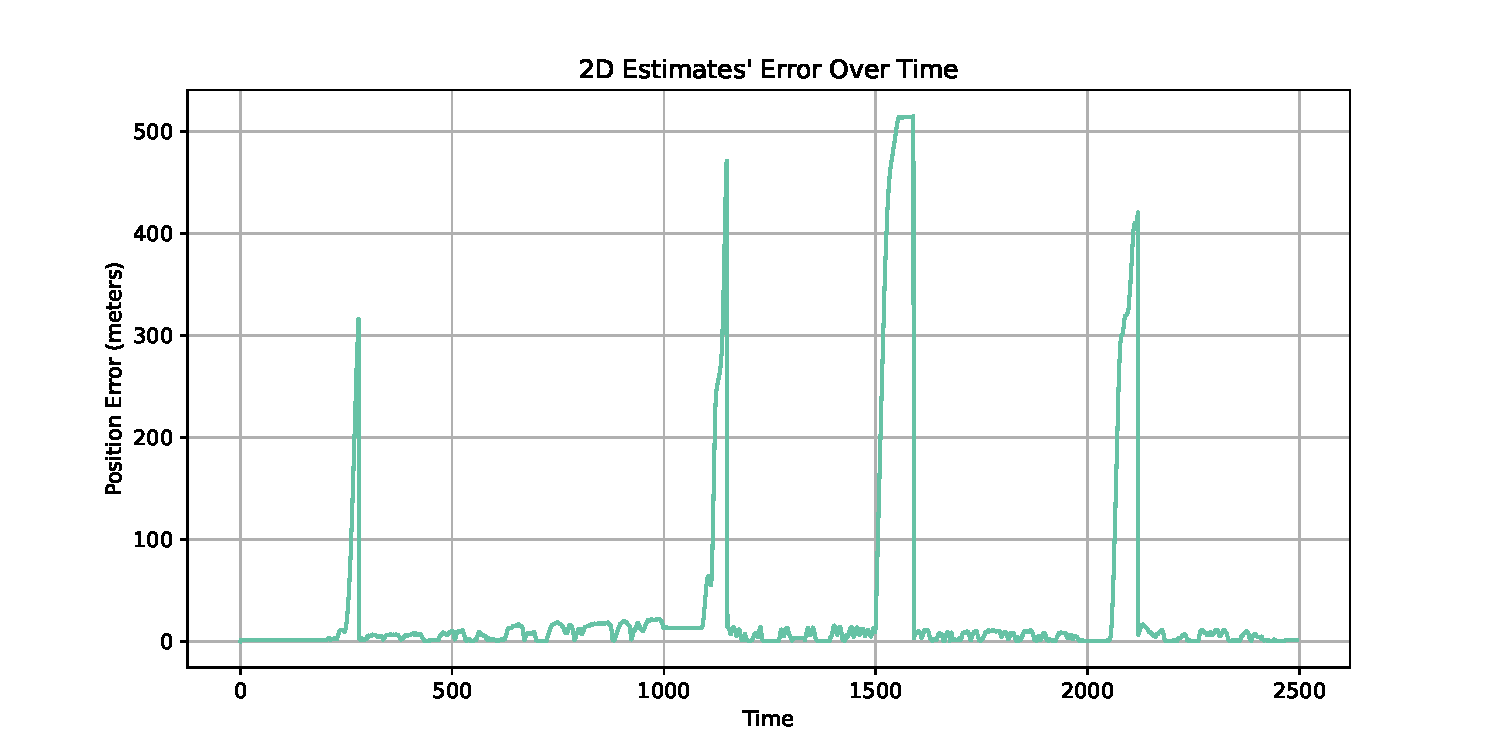
\includegraphics[width=0.48\textwidth]{plots/out2Derr.pdf}}
\caption{2D Positioning Errors in Presence of GPS Outages}
\label{fig:out_2D_err}
\end{figure}

Figure~\ref{fig:out_2D_err} illustrates the effect of GPS outages on 2D positioning. This analysis highlights the extent of drift in the absence of GPS corrections.

\section{Discussion}

\subsection{System Performance Under Normal Conditions}

\subsubsection{Trajectory Accuracy and Long-Term Drift Mitigation}
Upon inspecting the estimated trajectory (Figure~\ref{fig:traj}), we observe a tight alignment between the reference trajectory and the fused estimate. The GNSS corrections effectively mitigate the long-term drift inherent in inertial sensors, ensuring that the estimated path remains well-constrained over time. This result highlights the effectiveness of the Kalman filter fusion strategy, where the short-term precision of the INS is complemented by the absolute positioning capability of GNSS.

\subsubsection{Horizontal Positioning Accuracy and Error Trends}
Despite the strong overall agreement, deviations in horizontal positioning are noticeable, particularly in sharp turns or complex maneuvers.

Nevertheless, the RMS error for 2D (horizontal) positioning is approximately 8 meters, which suggests that the system achieves a reasonable level of accuracy for real-world navigation applications.

\subsubsection{Altitude Estimation and Vertical Positioning Challenges}
Altitude errors appear relatively stable, though occasional spikes are observed in the altitude error plot (Figure~\ref{fig:pos_err}). These fluctuations can be attributed to:
\begin{itemize}
    \item RISS's inherent limitations in altitude estimation, as it primarily relies on odometry and limited sensor redundancy for altitude tracking.
    \item GNSS altitude estimates are susceptible to degradation in instances of high Vertical Dilution of Precision (VDOP), leading to periods of increased vertical error.
\end{itemize}

\subsubsection{3D Positioning Error}
From Figure~\ref{fig:2D3D_err}, we see that the variability in 3D positioning error is largely influenced by deviations in 2D positioning. Since the horizontal error dominates, the overall 3D accuracy remains largely constrained by how well the system performs in 2D space.

\subsubsection{Velocity Estimation Performance}

Horizontal velocity estimates (East and North) are accurate, with errors generally below 1 m/s. 
Vertical velocity estimates exhibit more spikes, primarily due to the aforementioned altitude estimation challenges. 

Despite these challenges, the velocity errors remain within expected thresholds, ensuring that the system can deliver reliable motion state estimation across different navigation scenarios.

\subsection{Performance Under GPS Outages}

\subsubsection{INS Drift Accumulation During GPS Outages}
When GNSS updates are lost, the navigation system relies solely on dead reckoning using inertial sensors and odometry. As expected, the position errors grow rapidly, particularly in the latitude and longitude components, due to the absence of absolute position corrections. The 2D positioning error reaches values exceeding 300–500 meters in the longer GPS outages, demonstrating the well-known drift characteristic of INS-based navigation.

This behavior aligns with the expected error propagation in inertial navigation, where even small sensor biases and noise accumulate over time, leading to significant positional drift.

\subsubsection{Error Growth Over Time}
A key observation from the error trends is that the rate of error accumulation increases with longer outage durations. This is because the INS solution operates on recursive integration of accelerometer and gyroscope outputs, causing exponential-like error growth over time.

\begin{itemize}
    \item \textbf{Shorter outages} (~90–150 seconds) still result in notable drift, but the position estimates remain within a few hundred meters of the ground truth.
    \item \textbf{Longer outages} (\(\geq 3\) minutes) lead to substantial positioning errors, where the system's estimated trajectory significantly deviates from reality, demonstrating the inherent limitations of INS without external corrections.
\end{itemize}

This trend confirms that \textbf{INS-only navigation is unsuitable for extended GNSS-denied environments}, reinforcing the \textbf{importance of external updates} from GNSS or alternative aiding sensors.

Once GNSS updates resume, the Kalman filter recovers and corrects the accumulated errors, significantly reducing position drift. 

\section{Conclusion}

In this work, we presented a loosely coupled 3D RISS/GNSS integration system, demonstrating its performance under both nominal conditions and GNSS outages. Through a series of experiments and evaluations, we analyzed the system's positioning and velocity accuracy, as well as its ability to recover from GNSS signal losses.

Under normal conditions, the system exhibited strong agreement between the estimated and reference trajectories, with GNSS corrections effectively mitigating long-term inertial drift. The horizontal positioning accuracy achieved an RMS error of approximately 8 meters, which is suitable for real-world navigation applications. Velocity estimates remained highly accurate in the horizontal plane, with errors generally below 1 m/s, while altitude estimation faced moderate fluctuations due to GNSS VDOP variations and inherent limitations of RISS-based altitude tracking.

During GNSS outages, the system exhibited the expected dead reckoning drift, with 2D positioning errors exceeding 300–500 meters in extended outages. The longer the outage, the greater the accumulated drift, as errors compounded due to the recursive nature of INS integration. Upon GNSS restoration, the Kalman filter was able to correct the accumulated drift.

These findings reinforce the strengths of INS/GNSS fusion, particularly in combining the short-term accuracy of INS with the long-term stability of GNSS. However, the results also highlight areas for potential improvements, such as:
\begin{itemize}
    \item Tighter coupling strategies to allow partial GNSS updates even in degraded conditions.
    \item Integration of additional aiding sensors (e.g., barometers, odometry, LiDAR) to enhance robustness in extended GNSS-denied environments.
\end{itemize}

Overall, this study demonstrates that loosely coupled 3D RISS/GNSS integration provides a reliable navigation solution, but further refinements can enhance its resilience to prolonged GNSS outages. Future work will focus on improving outage robustness, refining the filtering model, and exploring additional sensor fusion techniques to advance INS/GNSS-based navigation for real-world applications.

\begin{thebibliography}{00}

\bibitem{iqbal2009} U. Iqbal, T. B. Karamat, A. F. Okou, and A. Noureldin, 
``Experimental Results on an Integrated GPS and Multisensor System for Land Vehicle Positioning,'' 
\textit{International Journal of Navigation and Observation}, Jun. 2009.

\bibitem{noureldin2013} A. Noureldin, T. B. Karamat, and J. Georgy, \textit{Fundamentals of Inertial Navigation, Satellite-Based Positioning and Their Integration}. Berlin, Germany: Springer-Verlag, 2013. 

\end{thebibliography}

\end{document}
